\documentclass{article}
\usepackage[utf8]{inputenc}

\usepackage[margin=1in,includefoot]{geometry}
\usepackage{fancyhdr}
\usepackage{mathmacros}

\fancyhead[L]{Measure Theory}
\fancyhead[R]{Alan Sun}
\fancyhead[c]{Chapter 3A: Integration with Respect to a Measure}
\fancyfoot{}

\fancyfoot[R]{\thepage}
\pagestyle{fancy}

\fancypagestyle{firstpage}{ \fancyfoot[L]{
    \emph{Measure, Integration, and Real Analysis by Sheldon Axler}
}}

\usepackage{tcolorbox}
\tcbuselibrary{breakable}
\usepackage{amsmath}
\usepackage{amssymb}
\usepackage{amsthm}
\usepackage{mathtools}
\usepackage{mathrsfs}
\usepackage{times}
\usepackage{enumitem}
\usepackage{wasysym}
\usepackage{newtxtext, newtxmath}

\newcommand{\eps}{\varepsilon}
\theoremstyle{remark}
\newtheorem{claim}{Claim}
\newenvironment{poc}{\textit{Proof of claim.}}{\qed\\}
\newtheorem{theorem}{Theorem}
\newtheorem{lemma}[theorem]{Lemma}

\newlist{legal}{enumerate}{10}
\setlist[legal]{label*=\arabic*.}


\begin{document}
\thispagestyle{firstpage}
\begin{enumerate}[leftmargin=*]
    \item[3.] We first show the ``if'' direction, \begin{claim}
        If $\mu(\{x \in X: f(x) > 0\}) > 0$, then $\int f \dd\mu > 0$.
    \end{claim}
    \begin{poc}
        Since $f$ is $\cS$-measurable, it must be that $f^{-1}((0,\infty]) \in \cS$. Thus,
        consider the $\cS$-partition defined by $A_1 = f^{-1}((0,\infty])$ and $A_2 = X \setminus A_1$.
        It follows that $\cL(f;A_1,A_2) > 0$ since $\mu(A_1) > 0$, by assumption. Then, from the 
        definition of the lebesgue integral, we have that $\int f\dd\mu \geq \cL(f;A_1,A_2) > 0$. 
    \end{poc}
    Now, for the converse.
    \begin{proof}
        Suppose that $\int f \dd\mu > 0$. Then, by the definition of the lebesgue integral, there
        exists a $\cS$-partition $A_1, \ldots, A_n$ such that $\cL(f;A_1,\ldots,A_n) > 0$. From the 
        definition of the lower lebesgue sum, 
        \[
            \cL(f;A_1,\ldots,A_n) = \sum_{k=1}^n \mu(A_k)\inf_{A_k} f > 0.
        \]
        Thus, there must exist some $A_k$ such that $\int_{A_k} f > 0$ and $\mu(A_k) > 0$. 
        Hence, by the subadditivty of $\mu$, $0 < \mu(A_k) \leq \mu(\{x \in X: f(x) > 0\})$.
    \end{proof}

    \item[4.] Consider the following function:
    \[
        f(x) = \begin{cases}1 &\text{if}\,x\notin\Q, \\ \frac{1}{n} &\text{if}\,x\in \Q\,\text{and}\,x=\frac{m}{n}.\end{cases}    
    \]
    I first show that this function must be Borel measurable. It suffices to show that for any $a \in \R$, 
    $f^{-1}((a,\infty))$ is a Borel set. If $a \geq 1$, then $f^{-1}((a,\infty)) \subset \Q$. Thus, it must be a Borel set.
    On the other hand, if $a < 1$, then $f^{-1}((a,\infty))$ contains all irrational numbers and a subset of all of the 
    rational numbers. This is also a Borel set, since it is $\R \setminus A$, where $A \subset \Q$. Thus, $f$ is Borel measurable.
    
    Now, consider any tagged partition, $a_0, a_1, \ldots, a_n$ such that $a_0 = 0, a_n = 1$ and $a_i < a_j$ for $i < j$. 
    Then, it follows that there must exist an irrational number in each $(a_i, a_j)$ for $i < j$. Thus, 
    $\inf_{(a_i,a_j)} f = 0$ (this follows directly from the proof that Thomae's function is continuous at all irrational numbers).
    Thus, $L(f,[0,1]) = 0$. 
    \item[5.] If $\sum_{k=1}^\infty b_k = \infty$, then consider any $\cS$-partition: $\{1\}, \{2,3,\ldots\}$.
    It follows that 
    \[
        \cL(f; \{1\}, \{2,3,\ldots\}) = b_1 + \mu(\{2,3,\ldots\})\inf {\{b_2,b_3,\ldots\}} = b_1 + \infty = \infty.
    \]
    Thus, by the definition of the lebesgue integral, it must be that 
    \[
        \int f \dd\mu \geq \infty.   
    \]
    Now, consider the case where $\sum_{k=1}^\infty b_k < \infty$. Then, it must be that $\lim_{k\to\infty} b_k = 0$. 
    Thus, for any $\cS$-partition, $A_1, A_2,\ldots$, there must exist a set $A_k$, in the $\cS$-partition such that $\mu(A) = \infty$
    and $\inf_A f = 0$. Hence, 
    \[
        \cL(f;A_1,A_2,\ldots) = \sum_{k \in \{A_i\}_{i\neq k}} b_k.
    \]
    So, taking the supremum over all such $\cS$-partitions, we have that 
    \[
        \int f \dd\mu \geq \sum_{k=1}^\infty b_k.
    \]
    \item[8.] Let $f_k$ be defined as follows:
    \[
        f_k(x) = \begin{cases}\frac{1}{k} &\text{if}\,x\in \left(-\frac{k}{2}, \frac{k}{2}\right), \\ 0 &\text{o/w}.\end{cases},
    \]
    for $k\in\Z^+$. Trivially, $f_k$ is Borel measurable. And it must also be that $\lim_{k\to\infty} f_k(x) = 0$ for any $x\in\R$. Now,
    consider the following claim.
    \begin{claim}
        For any $k\in\Z^+$, $\int f_k \dd\lambda = 1$. 
    \end{claim}
    \begin{poc}
        Consider the Borel-partition, $(-k/2, k/2), \R \setminus (-k/2, k/2)$. It follows that $\cL(f_k; (-k/2, k/2), \R \setminus (-k/2, k/2)) = 1$.
        Thus, $\int f_k \dd\lambda \geq 1$. On the other hand, consider any Borel-partition, $A_1, \ldots, A_n$. It follows that 
        \begin{align*}
            \cL(f_k; A_1,\ldots,A_n) &= \sum_{i=1}^n \lambda(A_i)\inf_{A_i} f_k, \\
            &= \sum_{\substack{i = 1 \\ A_i \subset (-k/2,k/2)}}^n \lambda(A_i)\inf_{A_i} f_k, \\
            &\leq \mu((-k/2,k/2)) \cdot \frac{1}{k} = 1.
        \end{align*}
    \end{poc}
    Thus, by claim 2, it follows that $\lim_{k\to\infty} \int f_k \dd\lambda = 1$. 
    \item[17.] \begin{enumerate}[label=(\alph*)]
        \item We have already shown that for any sequence of $\cS$-measurable functions, $f = \sup\{f_k\}_{k=1}^\infty$ and $g = \inf\{f_k\}_{k=1}^\infty$
        are both $\cS$-measurable. Thus, it follows from the definition of $\liminf$, for any $k\in\Z^+$, $g_k = \inf\{f_i\}_{i=k}^\infty$
        is $\cS$-measurable. Since each $g_k$ is measurable, then $f = \sup \{g_k\}_{k=1}^\infty$ is also measurable. Therefore, 
        $\liminf_{k\to\infty} f_k$ is measurable.
        \item Let $f'$ be defined such that $f_k'(x) = \inf_{k,k+1,\ldots} f_k(x)$. Then, it follows that $f_1', f_2', \ldots$ is a sequence 
        of increasing functions such that $f(x) = \lim_{k\to\infty} f_k'(x)$. And since each function is nonnegative, by the monotone convergence theorem, 
        it follows that $\int f \dd\mu = \lim_{k\to\infty} \int f_k'\dd\mu$. It remains to show that $\lim_{k\to\infty} \int f_k'\dd\mu \leq \liminf_{k\to\infty} \int f_k \dd\mu$.
        \begin{claim}
            $\lim_{k\to\infty} \int f_k' \dd\mu \leq \liminf_{k\to\infty} \int f_k \dd\mu$. 
        \end{claim}
        \begin{poc}
            Fix $k \in \Z^+$, then it must be that $\inf_{i \geq k} f_i \leq f_j$ for any $j \geq k$. Thus, since the lebesgue integral preserves order,
            it must be that 
            \[
                \int \inf_{i \geq k} f_i \dd\mu \leq \int f_j \dd\mu,  
            \]
            for any $j \geq k$. This implies that 
            \[
                \int \inf_{i \geq k} f_i \dd\mu \leq \inf_{i \geq k} \int f_i \dd\mu \leq \int f_j \dd\mu,  
            \]
            for any $j \geq k$. 
        \end{poc}
    \end{enumerate}
    \item[20.] For any $\eps > 0$, it suffices to show that there exists $N \in \Z^+$ such that for any $n > N$, 
    \[
        \left|\int f_k \dd\mu - \int f \dd\mu \right| < \eps. 
    \]
    From the definition of the real-Lebesgue integral, since each $f_k: X \to [-\infty, \infty]$,
    \begin{align*}
        \lim_{k \to \infty} \int f_k \dd\mu &= \lim_{k \to \infty} \int \underbrace{f_k^+}_{\text{(a)}} \dd\mu - \lim_{k \to \infty} \int \underbrace{f_k^-}_{\text{(b)}} \dd\mu,
    \end{align*}
    where if the sequence of functions $f_1, f_2, \ldots$ is increasing, then (a) is an increasing sequence of functions and (b) is a decreasing sequence of functions. On the other hand, 
    if the sequence of functions $f_1, f_2, \ldots$ is decreasing, then (a) is decreasing and (b) is increasing. Note that the monotone convergence theorem which we already proved covers 
    the case of the sequence of functions being increasing. Thus, it suffices to show that if the sequence of functions is decreasing, and its Lebesgue integral is bounded, then 
    interchanging of limits can be performed. First, consider the following claim,
    \begin{claim}\label{claim:eps}
        If $f: X \to [0, \infty]$ and $\int f \dd\mu < \infty$, then for every $\eps > 0$, there exist $E \in \cS$ (the $\sigma$-algebra of $X$) such that 
        $\mu(E) < \infty$ and \[
            \int \bigchi_{X \setminus E}f \dd\mu < \eps.     
        \]
    \end{claim}
    \begin{poc}
        By the definition of the Lebesgue integral, there exists a lower Lebesgue sum $\cL(f; \{A_i\}_{i=1}^n)$ such that 
        \[
            \int f \dd\mu < \cL(f; \{A_i\}_{i=1}^n) + \eps.
        \]
        Thus, let $E$ be the union of all $A_i$ such that $\inf_{A_i} f > 0$. Then, it follows that $\mu(E) < \infty$, otherwise $\int f \dd\mu = \infty$. 
        It also must follow that 
        \begin{align*}
            \int \bigchi_{E}f \dd\mu &\geq \cL(f; \{A_i\}_{i=1}^n), \\
            \int f\dd\mu - \int \bigchi_{E} f \dd\mu &< \eps, \\
            \int \bigchi_{X \setminus E} f \dd\mu &< \eps.
        \end{align*}
    \end{poc}
    Now, we show the central claim. Assuming that $\int |f_1| \dd\mu < \infty$, and $f_1, f_2, \ldots$ is a decreasing sequence of functions that converge pointwise to $f$ and $f_k: X \to [0,\infty]$. I 
    show that $\lim_{k\to\infty} f_k \dd\mu = \int f \dd\mu$. Let $\eps > 0$ be given.
    Using claim~\ref{claim:eps}, choose $E$ such that $\int_{X \setminus E} f_1 \dd\mu < \eps / 4$. Then, it follows that 
    \begin{align*}
        \left|\int f_k \dd\mu - \int f \dd\mu\right| &= \left|\int_{X \setminus E} f_k \dd\mu + \int_{E} f_k \dd\mu - \int_{X \setminus E} f \dd\mu + \int_E f \dd\mu \right|, \\
        &\leq \left|\int_{X \setminus E} f_k \dd\mu\right| + \left|\int_{X\setminus E} f\dd\mu \right| + \int_E |f_k - f| \dd\mu, \\
        &< \frac{\eps}{2} + \mu(E) \sup_{x \in E} |f_k(x) - f(x)|.
    \end{align*}
    By Egorov's theorem, $f_k$ converges uniformly to $f$ on $E$. Thus, since $\mu(E)$ is finite, $\mu(E) \sup_{x\in E} |f_k(x) - f(x)|$ can be arbitrarily small.
    \item[21.] First, let's consider the Riemann integral. Let $f$ be a Riemann integrable function on $[a,b]$.
    Then, it follows that $\int_a^b f(x) \dd x$ is the supremum over all partitions of $[a,b]$ of the lower Riemann sums.
    Note that we start with a partition, then sum according to the partitions. See Fig.~\ref{fig:riemann} for an example.
    \begin{figure}
        \centering
        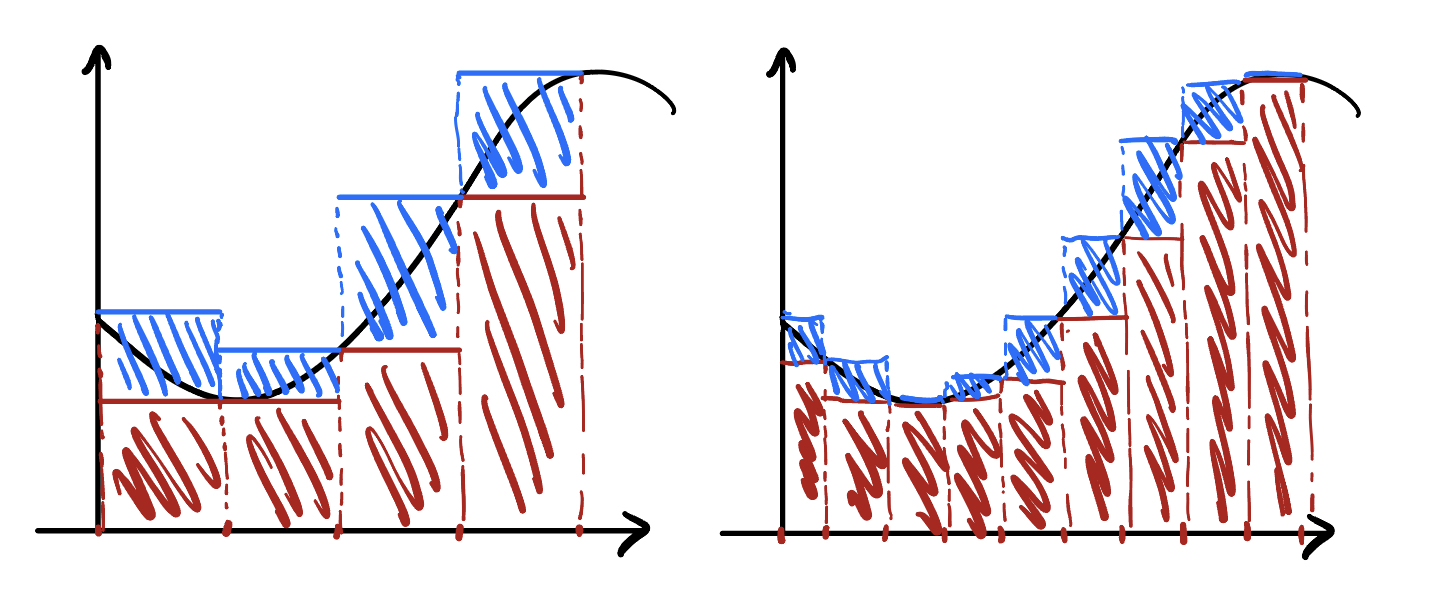
\includegraphics[width=0.8\textwidth]{riemann.jpeg}
        \caption{The upper and lower sums of a Riemann integrable function.}
        \label{fig:riemann}
    \end{figure}
    In this way, the Riemann integral partitions the domain of the function. On the other hand, the lebesgue integral partitions the range of the function.
    Suppose that $f: X \to [0,\infty]$ is $\cS$-measurable, there exists simple, measurable functions $f_1, f_2,\ldots$ that 
    converge pointwise to $f$. For each of these simple measurable functions, $f_k = \sum_{i=1}^n c_i\chi{A_i}$,
    the lebesgue integral is simply
    \[
        \int f_k \dd\lambda = \sum_{i=1}^n c_i \lambda(A_i),
    \]
    as we proved in the text. Note that the coefficients $c_i$ partition the range of $f$. Thus, the lebesgue integral partitions the range of the function.
    can be thought of as partitioning the range. See Fig.~\ref{fig:lebesgue} for an example.
    \begin{figure}
        \centering
        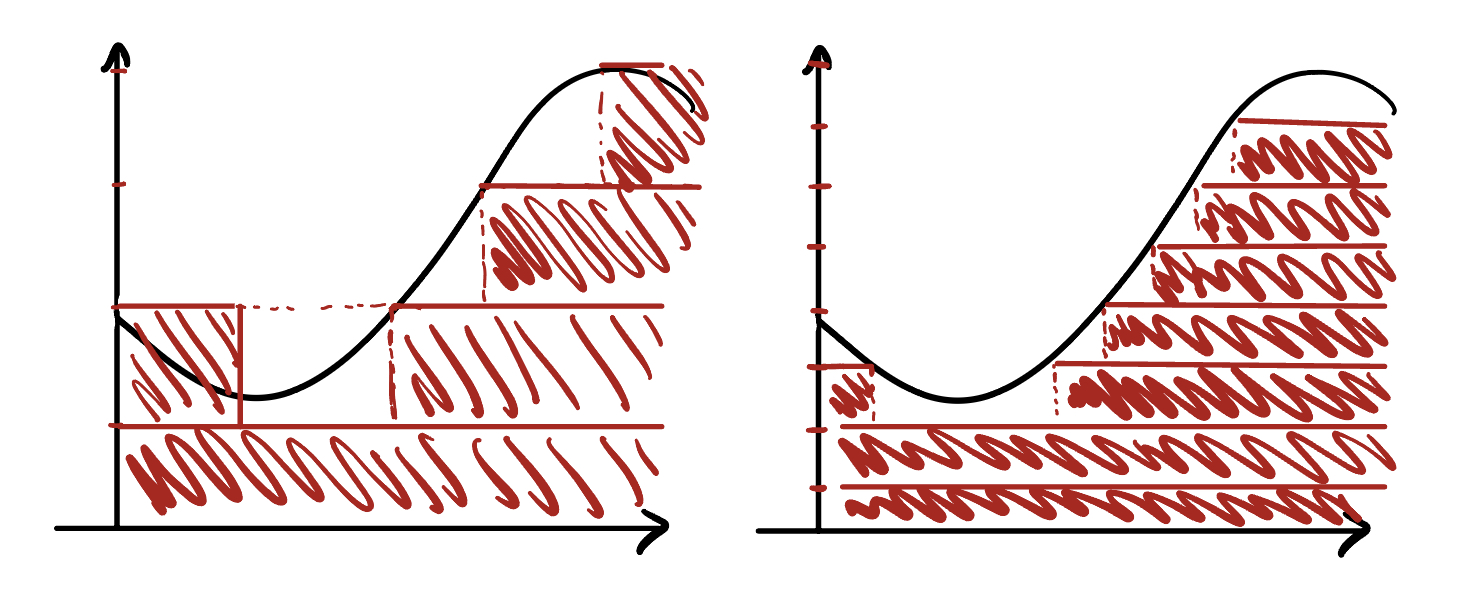
\includegraphics[width=0.8\textwidth]{lebesgue.jpeg}
        \caption{The integral of a measurable function being approximated by a sequence of simple measurable 
        functions that converge pointwise to the desired function.}
        \label{fig:lebesgue}
    \end{figure}
\end{enumerate}
\end{document}
